\documentclass[a4paper,11pt,english]{article}
\usepackage[T1]{fontenc}
\usepackage[utf8]{inputenc}
\usepackage{lmodern}
\usepackage{graphicx}
\usepackage{babel,blindtext}
\usepackage{float}
\usepackage{wrapfig}	
\title{PH21 Assignment 5 v2: last section updated}
\author{Helen Xue}


\begin{document}

\maketitle


\section{Coin}
\par I used pymc to generate the following plots/distributions, with a chain length of 10k:
\par True probability = 0.4:
\begin{figure}[H]

	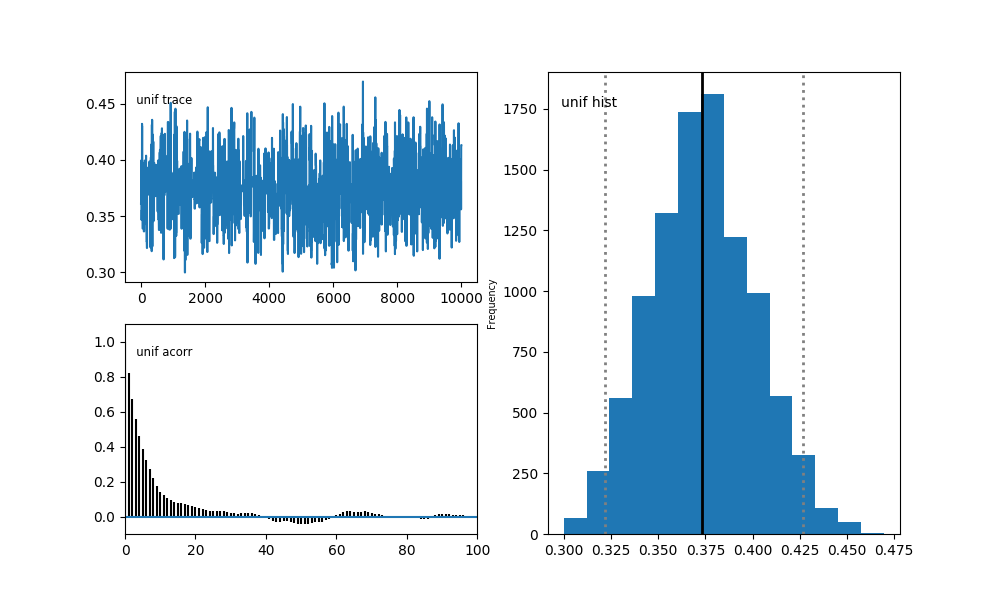
\includegraphics[width=\linewidth]{coin/unif}
	uniform prior coin toss ;   95$\%$ confidence interval: [0.322 0.427]
	
	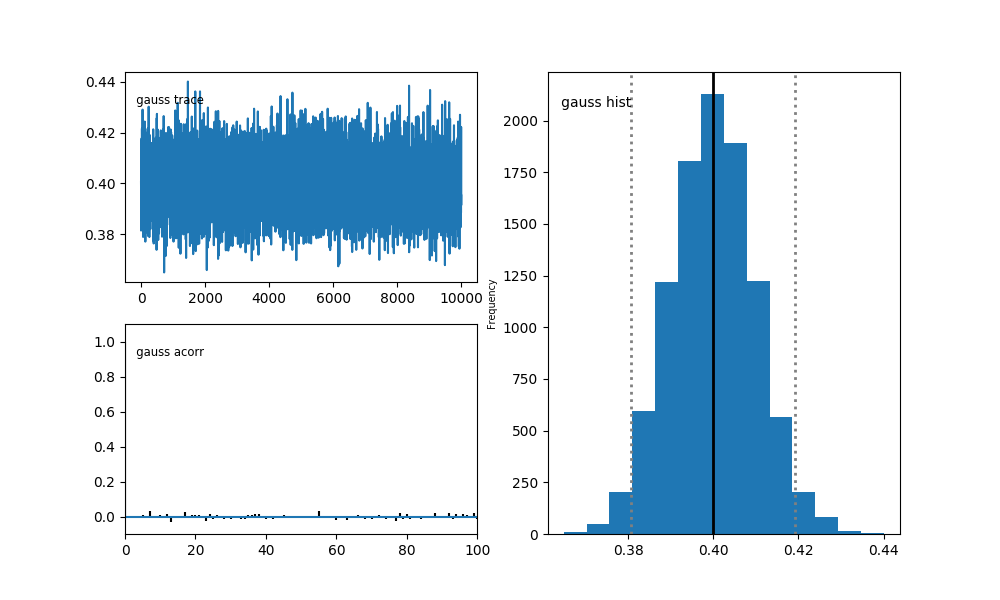
\includegraphics[width=\linewidth]{coin/gauss}
	gaussian prior coin toss ;  95$\%$ confidence interval: [0.395 0.503]
\end{figure}

\par The uniform prior consistently did not converge on the right interval as quickly, even when I increased the chain length to; this is because the uniform prior has more variation.  The trace amplitude is larger, and the peak is less crisp.
\par Varying the bias value for the gaussian prior threw off the results, depending on how much variation we allowed.

\section{Lighthouse: updated}
\par Updates: I increased the chain length to 100k and increased the burning period and thinning interval to reduce autocorrelation. We can see that there's minimal autocorrelation from the plots, and the results are much nicer; both confidence intervals center on the true values, and the results appear to converge relatively quickly.		 
\par True b = 1.5:
\begin{figure}[H]
	
	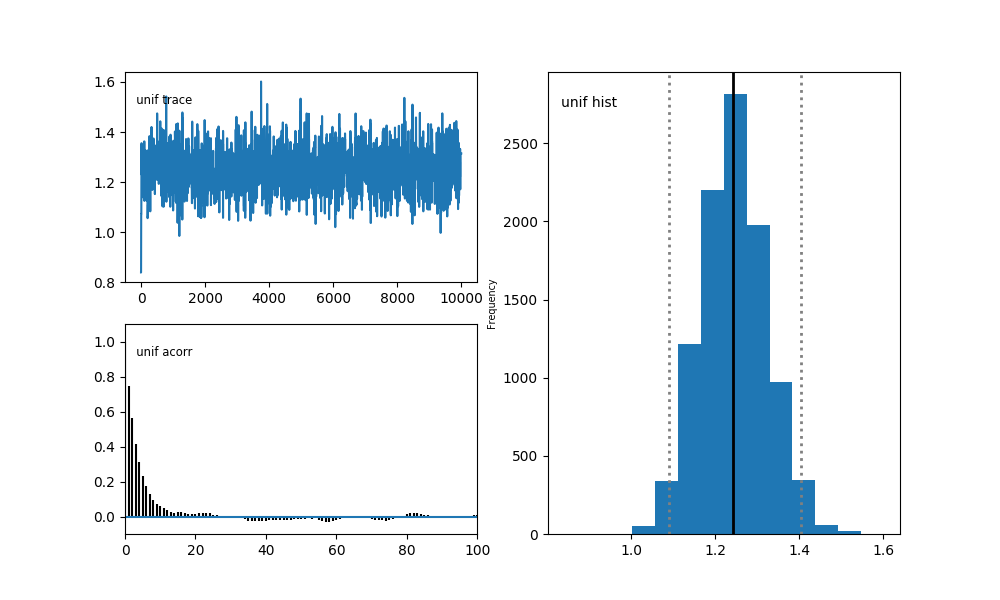
\includegraphics[width=\linewidth]{lighthouse/b_unif}
	uniform prior coin toss ;   95$\%$ confidence interval: [1.241 1.7  ]
	
	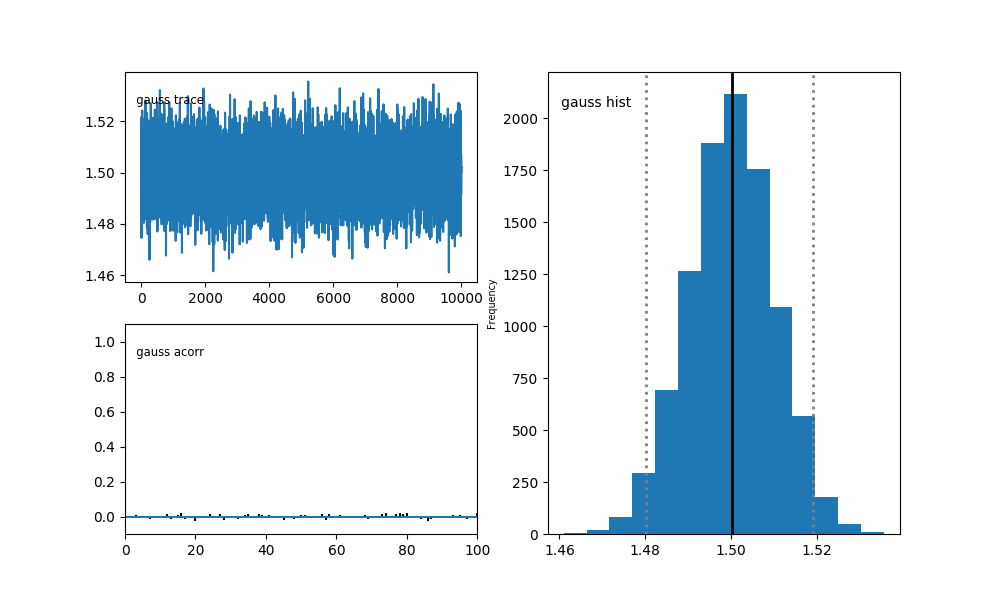
\includegraphics[width=\linewidth]{lighthouse/b_gauss}
	gaussian prior coin toss ;  95$\%$ confidence interval: 
[1.207 1.626]
	
\end{figure}

\par True a = 1.0:
\begin{figure}[H]
	
	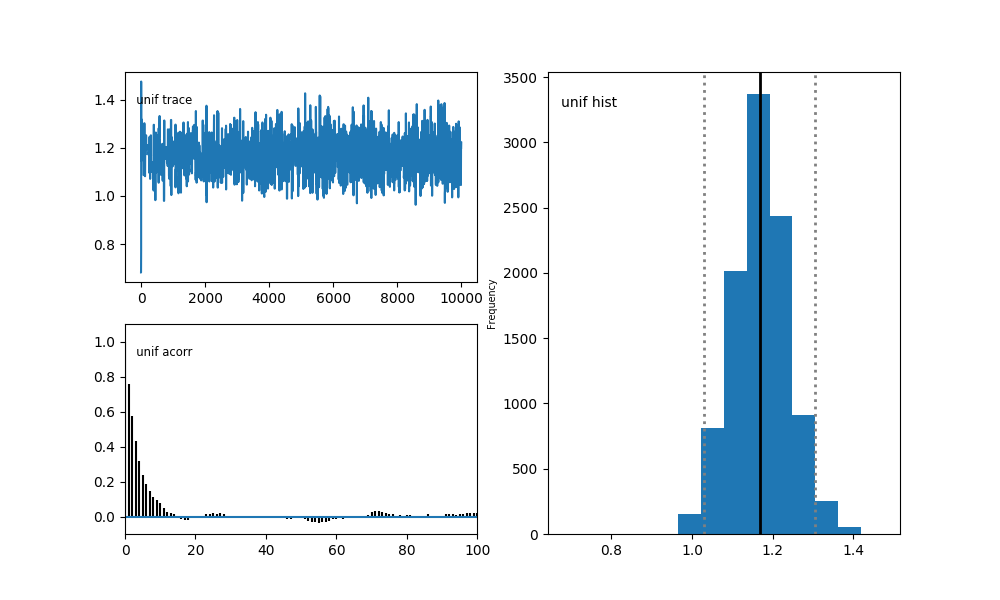
\includegraphics[width=\linewidth]{lighthouse/a_unif}
	uniform prior coin toss ;   95$\%$ confidence interval:  [0.813 1.249]
	
		
	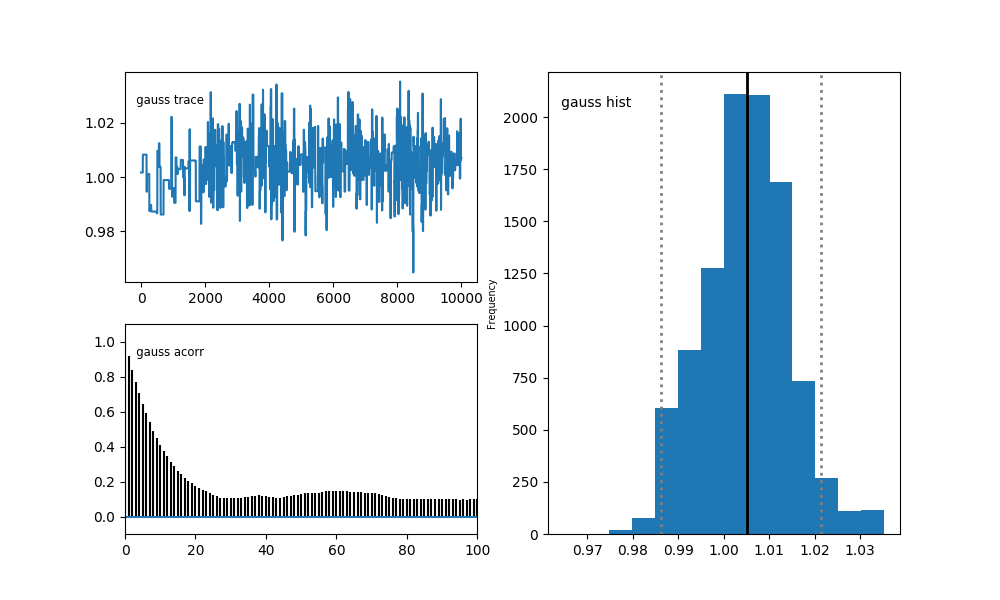
\includegraphics[width=\linewidth]{lighthouse/a_gauss}
	gaussian prior coin toss ;  95$\%$ confidence interval: 
[0.721 1.135]


\end{figure}

\end{document}
